\documentclass[12pt, letterpaper, oneside]{article}
\usepackage[nolinks]{qrcode}
\usepackage[absolute,overlay]{textpos}
\usepackage[letterpaper,  left=30mm, right = 30mm, top=40mm, bottom=20mm]{geometry}                		
\usepackage{graphicx}
\usepackage{tikz}
\usetikzlibrary{calc,through,intersections, arrows, shapes, decorations.markings, matrix, patterns}
\usepackage{enumitem}

\usepackage{pifont}
\usepackage[math]{iwona}

%%% PARSKIP AND PARINDENT 
\setlength{\parindent}{0in}
\setlength{\parskip}{0mm}


\begin{document} 

\thispagestyle{empty}

%---------------------------------------------------
%  TITLE PAGE
%---------------------------------------------------


\thispagestyle{empty}
\newgeometry{left=10mm, right=10mm, top=40mm, bottom=20mm} 

\ 

\begin{center}
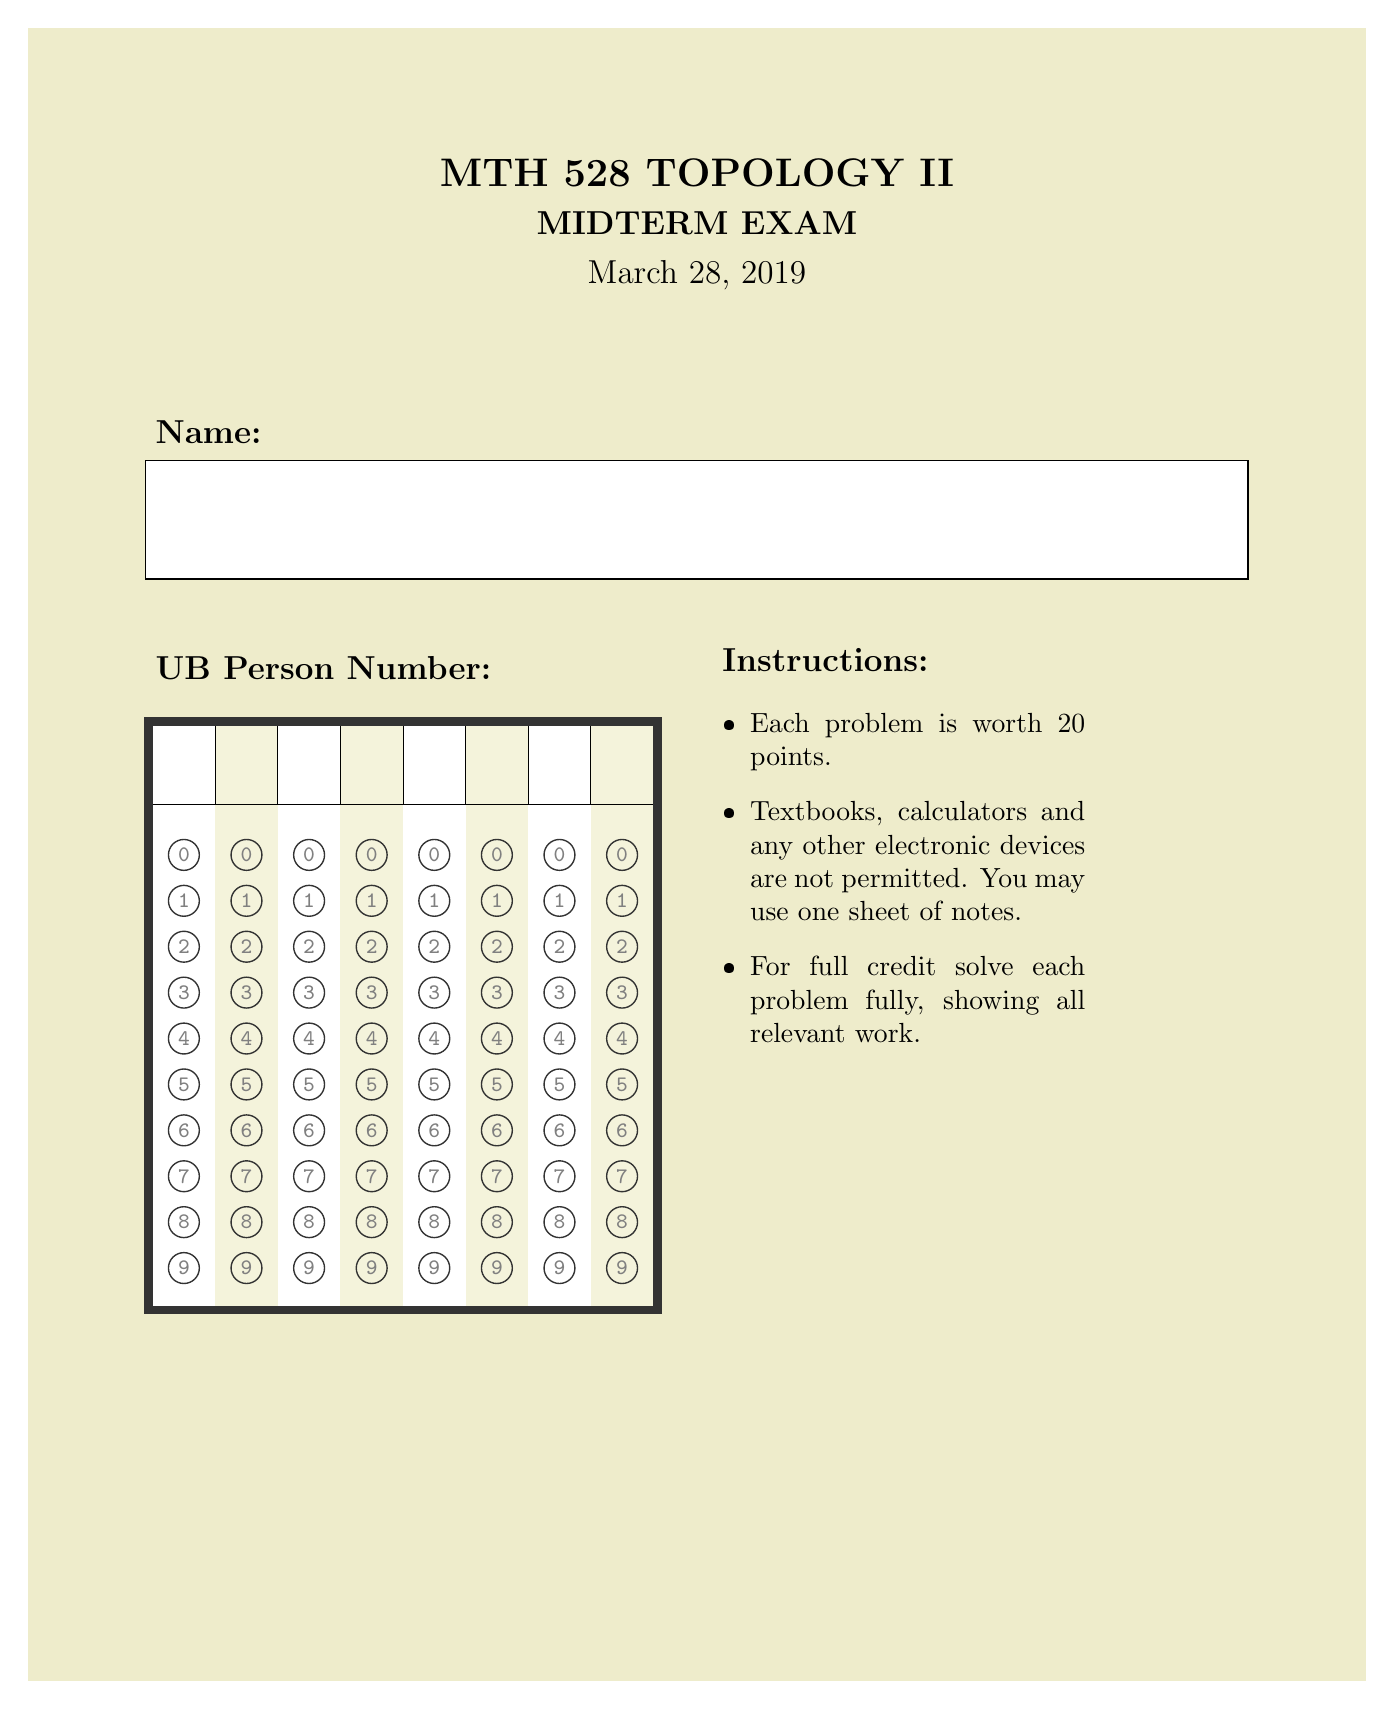
\begin{tikzpicture}
%background and header
\fill[olive!15] (-0.5,0) rectangle (16.5, 21);
\node at (8, 18.5) {\begin{minipage}{\textwidth}
\begin{center}
{\Large \bf{MTH 528 TOPOLOGY II}}\\[2mm]
{\large \bf{MIDTERM EXAM}} \\[2mm]
 {\large March 28, 2019} \\
\end{center}
\end{minipage}
};

% name box
\node[anchor = south west] at (1, 15.6) {\large \bf Name:};
\draw[fill  = white, line width = 0.5]  (1, 14) rectangle +(14, 1.5);



% person number
\node[anchor = south west] at (1, 12.6) {\large \bf UB Person Number:};

\begin{scope}[scale=0.53, yshift = 200mm, xshift =13mm]
\draw[black!50, fill = white, line width = 3]  (0.65, 3) rectangle +(8*1.5 + 0.2, -1.1*11-2);

\foreach \x in {1,3,5,7}{
\fill[olive!10]  (0.75 + 1.5*\x, 3) rectangle +(1.5, -1.1*11 - 2);
};
\foreach \x in {1,...,8}{
\draw[line width = 0.3]  (1.5*\x-0.75, 1) rectangle +(1.5, 2);
}

\draw[black!80,  line width = 3]  (0.65, 3) rectangle +(8*1.5 + 0.2, -1.1*11-2);

\foreach \y [evaluate={\z=int(-1*\y);}] in {0,-1,...,-9}{
\foreach \x in {1,...,8}{
\draw[line width = 0.5, color=black!80 ] (1.5*\x, 1.1*\y- 0.2) circle (0.37);
\node at (1.5*\x, 1.1*\y - 0.2) {\footnotesize \color{black!50}\tt \z};
};
}
\end{scope}



% instructions
\node[anchor=north west] at (8.2, 13.24) {\begin{minipage}{0.38\textwidth}
{\large \bf Instructions:}


\begin{itemize}[leftmargin=*]
\item  Each problem is worth 20 points. 

\item Textbooks, calculators and any other electronic devices are not permitted. 
You may use one sheet of notes.  

\item For full credit solve each problem fully, showing all relevant work.
\end{itemize}  

\end{minipage}
};


\end{tikzpicture}
\end{center}

%% QR CODE
\begin{textblock*}{11cm}[1, 0](8.2in, 0.3in) % {block width} [anchor point] (coords) 

\begin{tikzpicture}
\draw[opacity = 0] (-8, 0) rectangle (2.2 , -2.2);
\node[fill=white, anchor= north west] at (0,0)
{\qrcode[height=25mm, level=H]{MTH-309T-F19-EX1-005-P00}};
\node[anchor =  north east] at (0, -1) {\large\tt \begin{tabular}{r} MTH-309T-F19-EX1-005-P00 \end{tabular}};
\end{tikzpicture}
\end{textblock*}
%% END QR CODE


\restoregeometry

%---------------------------------------------------
% END TITLE PAGE
%---------------------------------------------------


\newpage 


This is problem 1

%% QR CODE
\begin{textblock*}{11cm}[1, 0](8.2in, 0.3in) % {block width} [anchor point] (coords) 

\begin{tikzpicture}
\draw[opacity = 0] (-8, 0) rectangle (2.2 , -2.2);
\node[fill=white, anchor= north west] at (0,0)
{\qrcode[height=25mm, level=H]{MTH-309T-F19-EX1-005-P01}};
\node[anchor =  north east] at (0, -1) {\large\tt \begin{tabular}{r} MTH-309T-F19-EX1-005-P01 \end{tabular}};
\end{tikzpicture}
\end{textblock*}
%% END QR CODE

\newpage 

This is problem 2


%% QR CODE
\begin{textblock*}{11cm}[1, 0](8.2in, 0.3in) % {block width} [anchor point] (coords) 

\begin{tikzpicture}
\draw[opacity = 0] (-8, 0) rectangle (2.2 , -2.2);
\node[fill=white, anchor= north west] at (0,0)
{\qrcode[height=25mm, level=H]{MTH-309T-F19-EX1-005-P02}};
\node[anchor =  north east] at (0, -1) {\large\tt \begin{tabular}{r} MTH-309T-F19-EX1-005-P02 \end{tabular}};
\end{tikzpicture}
\end{textblock*}
%% END QR CODE


\end{document}
